% !TEX root = main.tex
%
% Correspondance between nested-words and trees

The hierarchical structure of nested words, defined with the \emph{call} 
and \emph{return} markup symbols
suggest a correspondence with trees.
The lifting of this correspondence to languages, of tree automata and VPA,
has been discussed in~\cite{AlurMadhusudan09nested},
and~\cite{Caralp12VPAmult} for the weighted case.
In this section, we describe a correspondence between the symbolic-weighted extensions
of tree automata and VPA.

Let $\Omega$ be a countable ranked alphabet, such that
every symbol $a \in \Omega$ has a rank
$\rank(a) \in [0..M]$ where $M$ is a fixed natural number.
We denote by $\Omega_k$ the subset of all symbols $a$ of $\Omega$
with $\rank(a) = k$, where $0 \leq k \leq M$,
and $\Omega_{>0} = \Omega \setminus \Omega_0$.
%
\noindent
The free $\Omega$-algebra of finite, ordered,
$\Omega$-labeled trees is denoted by $\T_\Omega$.
It is the smallest set such that  $\Omega_0 \subset \T_\Omega$
and for all $1 \leq k \leq M$, all $a \in \Omega_k$,
and all $t_1, \ldots, t_k \in \T_\Omega$, $a(t_1, \ldots, t_k) \in \T_\Omega$.
%
% tree = single node (leave) labeled with a symbol of $a \in \Omegai$
% (such a tree is simply denoted by $a$)
% or the composition, denoted by $b(t_1,\ldots, t_n$) of a node labeled with $b$
% and $n$ subtrees $t_1$,\ldots, $t_n$.
%
Let us assume a commutative semiring~$\Semiring$
and a label theory~$\bar{\Phi}$ over~$\Semiring$
containing one set~$\Phi_{\Omega_k}$ for each $k \in [0..M]$.
%
\renewcommand{\call}[1]{\ensuremath \langle_{#1}}
\renewcommand{\return}[1]{\ensuremath {}_{#1}{\rangle}} % $\prescript{}{a}{)}$

% A \emph{regular tree grammar} over $\Omega$
% is a triplet $G = \< N, q_\mathsf{i}, R>$ where
% $N$ is a finite set of non-terminal symbols denoted $q$...,
% $q_\mathsf{i} \in N$ is the starting non-terminal,
% $R$ is a finite set of production rules of the form
% $q_0 \to a(q_1\ldots q_k)$ where
% $q_0, q_1, \ldots, q_k \in N$
% $a \in \Omega_k$.
% A tree $t \in \T_\Omega$ is in the language of $G$
% if it can be generated from $q_\mathsf{i}$ by
% non terminal replacement following the rules of $R$.
%
\begin{definition}  \label{def:SWTA}
A \emph{symbolic-weighted tree automaton} (\SWTA)
over $\Omega$, $\Semiring$, and~$\bar\Phi$
is a triplet $A = \< Q, \init, \bar{\wei} >$ where
$Q$ is a finite set of states,
$\mathsf{in} : Q \to \Phi_\Omega$ is the starting weight function,
and $\bar{\wei}$ is a tuplet of transition functions containing,
for each $k \in [0..M]$,
%$\wei_\varepsilon$ from $Q \times Q$ into $\Semiring$, and,
the functions $\wei_{k}: Q \times Q^{k} \to \Phi_{\Omega_{>0},\Omega_k}$
and $\weie[k]: Q \times Q^{k} \to \Phi_{\Omega_k}$.
\end{definition}
%
%Like in Section~\ref{sec:SWAdef},
We define %from $\bar{\wei}$
a transition
function~$\wei: Q \times (\Omega_{> 0} \cup \{ \varepsilon \}) \times \Omega \times \bigcup_{k=0}^{M} Q^k
  \to \Semiring$
by: %also called $\wei$ for simplicity,
%such that, for all $q, q' \in Q$, $a \in \Sigma$, and $b \in \Delta$,
\[
\begin{array}{rcll}
%\wei(q_0, \varepsilon, q_1) & = &  \wei_\varepsilon(q_0, q_1),\\ %\phi_\varepsilon\\
\wei(q_0, a, b, q_1 \ldots q_k) & = & \eta(a, b) &
\quad\mathrm{where~} \eta = \wei_{k}(q_0, q_1\ldots q_k)\\
\wei(q_0, \varepsilon, b, q_1 \ldots q_k) & = & \phi(b) &
\quad\mathrm{where~} \phi = \weie[k](q_0, q_1\ldots q_k).
\end{array}
\]
%
\noindent
where $q_1\ldots q_k$ is $\varepsilon$ if $k = 0$.
The first case deals with a strict subtree, with a parent node labeled by $a$,
and the second case is for a root tree.

\noindent
Every \SWTA %of Definition~\ref{def:SWTA}
defines a mapping
from trees of $\T_\Omega$ into~$\Semiring$, %the weight values in~$\Semiring$,
based on the following intermediate function
$\weight_A: Q \times (\Omega \cup \{ \varepsilon \}) \times \T_\Omega \to \Semiring$
\begin{equation}
%\begin{array}{rccl}
\weight_A(q_0, a, t) =  % & = &
%   \displaystyle\bigoplus_{q_1 \in Q} &
%   \wei(q, \varepsilon, q_1) \otimes \weight_A(q_1, t)\\
 \displaystyle\bigoplus_{q_1 \ldots q_k \in Q^k} % &
              \wei(q_0, a, b, q_1 \ldots q_k )
   \otimes \displaystyle\bigotimes_{i=1}^{k}
           \weight_A(q_i, b, t_i)
%\end{array}
\end{equation}
where $q_0 \in Q$, $a \in \Omega_{>0} \cup \{ \varepsilon \}$ and
$t = b(t_1,\ldots, t_k) \in \T_\Omega$,
$0 \leq k \leq M$.

\medskip\noindent
Finally, the weight associated by $A$ to  $t \in \T_\Omega$ is
\begin{equation}
A(t)  =
\displaystyle\bigoplus_{q \in Q} \mathsf{in}(q) \mathop{\otimes} \weight_A(q, \varepsilon, t)
\label{eq:weightTA}
\end{equation}

\noindent
Intuitively, $\wei(q_0, a, b, q_1 \ldots q_k)$ can be seen as
the weight of a production rule $q_0 \to b(q_1, \ldots, q_k)$
of a regular tree grammar~\cite{tata},
that replaces the non-terminal symbol $q_0$ by $b(q_1, \ldots, q_k)$,
provided that the parent of $q_0$ is labeled by $a$
(or $q_0$ is the root node if $a = \varepsilon$).
%in a step of tree building.
%
%Such a grammar computes the weights of the derivation trees
%of the Context-Free grammar obtained by forgetting the labeling symbols of $\Omega_{>0}$.
The above production rule can also be seen as
a rule of a weighted CF grammar, of the form
$[a, b]\, q_0 := q_1 \ldots q_k$ if $k > 0$,
and $[a]\, q_0 := b$ if $k = 0$.
In the first case, $b$ is a label of the rule,
and in the second case, it is a terminal symbol.
And in both cases, $a$ is a constraint on the label of rule applied
on the parent node in the derivation tree.
This features of observing the parent's label
are useful in the case of infinite alphabet,
where it is not possible to memorize a label with the states.
%
%One can observe that
\noindent The weight of a labeled derivation tree $t$
of the weighted CF grammar associated to~$A$ as above,
is $\weight_A(q, t)$,
when $q$ is the start non-terminal.
%
We shall now establish a correspondence between such a derivation tree $t$
and some word describing a linearization of $t$,
in a way that $\weight_A(q, t)$ can be computed by a $\SWVPA$.

Let $\hat\Omega$ be the countable (unranked) alphabet obtained
from $\Omega$ by:
$\hat\Omega = \Deltai \uplus \Deltac \uplus \Deltar$, with
$\Deltai = \Omega_0$,
$\Deltac = \{ \; \call{a} \mid a \in \Omega_{>0} \}$,
$\Deltar = \{ \; \return{a} \mid a \in \Omega_{>0} \}$.

\noindent
We associate to $\hat\Omega$
a label theory $\hat{\Phi}$
like in Section~\ref{sec:SWVPA-def},
%
\noindent
and we define a linearization of trees of $\T_\Omega$ into
words of ${\hat\Omega}^*$ as follows:
\begin{description}
\item $\lin(a) = a$ for all $a \in \Omega_0$,
\item $\lin\bigl( b(t_1, \ldots, t_k)\bigr) =
       \call{b} \; \lin(t_1) \ldots \lin(t_k) \; \return{b}$
       when $b \in \Omega_k$ for $1 \leq k \leq M$.
\end{description}
%
\begin{example}
The trees in Figure~\ref{fig:score-tree}
represent the two scores in Examples~\ref{ex:running},\ref{ex:nested-word}, 
and their linearization are respectively~$O$ and~$O'$ inn the same examples.
\end{example}


\begin{proposition}\label{lem:SWTA}
For all \SWTA $A$ over~$\Omega$, $\Semiring$ commutative, and $\bar\Phi$,
there exists an effectively constructible \SWVPA $A'$ over
$\hat\Omega$, $\Semiring$ and $\hat\Phi$
such that for all $t \in \T_\Omega$, $A'\bigl(\lin(t)\bigr) = A(t)$.
\end{proposition}
%
\begin{proof}
Let $A = \< Q, \init, \bar{\wei} >$ where $\bar{\wei}$ is presented as above by a function
    %
We build
$A' = \< Q', P', \init', \bar{\wei}', \final' >$,
%computing over $\Delta = \Omegai \uplus \Omegac \uplus \Omegar$,
where $Q' = \bigcup_{k=0}^{M} Q^k$ is the set of sequences of state symbols of $A$,
of length at most $M$, including the empty sequence denoted by~$\varepsilon$,
and where $P' = Q'$ and $\bar\wei$ is defined by:

\[
\begin{array}{lcll}
\weii(q_0\, \bar{u}, {\call{c}}, \bar{p}, a, \bar{u}) & = & \wei(q_0, c, a, \varepsilon) &
\mathrm{for~all~} c \in \Omega_{>0}, a \in \Omega_0\\ %\bar{p}\in P',
%
\weiei(q_0\,\bar{u}, a, \bar{u}) & = & \wei(q_0, \varepsilon, a, \varepsilon) &
\mathrm{for~all~} a \in \Omega_0\\
%
\weic(q_0\,\bar{u}, {\call{c}}, \bar{p}, \call{d}, \bar{u}, \bar{q}) & = & \wei(q_0, c, d, \bar{q}) &
\mathrm{for~all~} c, d \in \Omega_{>0}\\ % \bar{p}\in P'
%
\weiec(q_0\,\bar{u}, \call{c}, \bar{u}, \bar{q}) & = & \wei(q_0, \varepsilon, c, \bar{q}) &
\mathrm{for~all~} c \in \Omega_{>0}\\
%
%\weir: Q \times \Omegac \times P \times \Sigmar \times Q \to \Semiring &
\weir(\varepsilon, {\call{c}}, \bar{p}, {\return{c}}, \bar{p}) & = & \one &
\mathrm{for~all~}  c \in \Omega_{>0}\\ % \bar{p}\in P'
%
%\weie: Q \times \Omegar \times Q \to \Semiring &
\weier(\bar{u}, {\return{c}}, \bar{q}) & = & \zero &
\mathrm{for~all~}  c \in \Omega_{>0}
\end{array}
\]
\noindent
All cases not matched by one of the above equations have a weight $\zero$,
for instance  %This is in particular the case of
$\weir(\bar{u}, {\call{c}}, \bar{p}, {\return{d}}, \bar{q}) = \zero$
if $c \neq d$
or $\bar{u} \neq \varepsilon$
or $\bar{q} \neq \bar{p}$.
%
%\noindent
%It is sufficient to consider in $Q'$ only the prefixes of
%sequences in transition with a non-null weight.
%\qed
\end{proof}

\begin{figure}
\begin{center}
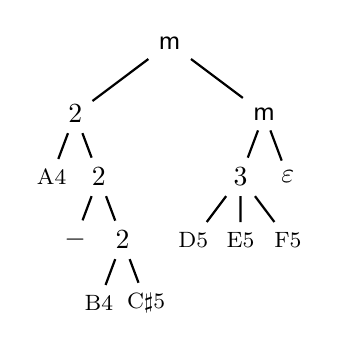
\begin{tikzpicture} [-,thick]
\tikzstyle{level 1}=[level distance=9mm,sibling distance=24mm]
\tikzstyle{level 2}=[level distance=8mm,sibling distance=6mm]
\tikzstyle{level 3}=[level distance=8mm,sibling distance=6mm]
\node {$\mathsf{m}$}
  child { node {$2$}
    child { node {$\mbox{\footnotesize A4}$} }
    child { node {$2$}
      child { node {$-$} }
      child { node {$2$}
        child { node {$\mbox{\footnotesize B4}$} }
        child { node {$\mbox{\footnotesize C$\sharp$5}$} }}}}
  child { node {$\mathsf{m}$}
    child { node {$3$}
      child { node {$\mbox{\footnotesize D5}$} }
      child { node {$\mbox{\footnotesize E5}$} }
      child { node {$\mbox{\footnotesize F5}$} }}
    child { node {$\varepsilon$} }};        
\end{tikzpicture}
%
\quad 
%
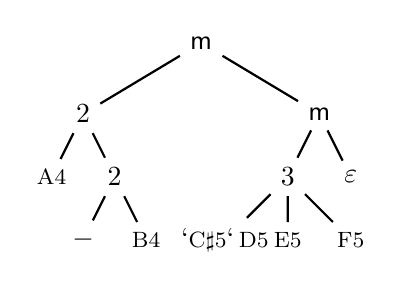
\begin{tikzpicture} [-,thick]
\tikzstyle{level 1}=[level distance=9mm,sibling distance=30mm]
\tikzstyle{level 2}=[level distance=8mm,sibling distance=8mm]
\tikzstyle{level 3}=[level distance=8mm,sibling distance=8mm]
\node {$\mathsf{m}$}
  child { node {$2$}
    child { node {$\mbox{\footnotesize A4}$} }
    child { node {$2$}
      child { node {$-$} }
      child { node {$\mbox{\footnotesize B4}$} } } }
  child { node {$\mathsf{m}$}
    child { node {$3$}
      child { node {$`\mbox{\footnotesize C$\sharp$5}`\,\mbox{\footnotesize D5}$} }
%                   {$\begin{array}{c}
%                     \mbox{\footnotesize C5}\\
%                     \mbox{\footnotesize D5}
%                     \end{array}$} }
      child { node {$\mbox{\footnotesize E5}$} }
      child { node {$\mbox{\footnotesize F5}$} } }
    child { node {$\varepsilon$} } };        
\end{tikzpicture}
\end{center}
\caption{Tree representation of scores 
of Examples~\ref{ex:running},\ref{ex:nested-word}, 
linearized respectively into~$O$ and~$O'$.}
\label{fig:score-tree}
\end{figure}

